\documentclass{article}
\usepackage[margin=0.5in]{geometry}
\usepackage[utf8]{inputenc}
\usepackage{graphicx}
\usepackage{amsmath}
\usepackage{cite}

\title{Harris Corner Detector and SIFT Descriptor}
\author{Toby Hijzen \& Kristin Rieping}
\date{\today}

\begin{document}

\maketitle

\section{Introduction}
To match images or objects in images to each other it is common practice to detect salient points in both images. This increases robustness and reduces complexity as well as the computational cost of matching. These feature points should be robust to rotation, scaling and changes in intensity. Good features that display these properties are corner points. Therefore the focus is on the detection of corners. This report shortly discusses three different methods for detecting corners. The first two are based on the Harris corner detection scheme whereas the third is based on the difference of gaussians (DoG) method. Finally the points of two images are matched to each other using David Lowes SIFT. The results of this are reported for each corner detector.

\section{Harris Corner Detector}
We implemented the Harris Corner Detector in Matlab. 
First we computed the cornerness $R$ for every point in the image with
\begin{equation}
R = \det(M) - k*(\mathrm{trace}(M))^2
\end{equation}
where $k=0.04$ is a constant and
\begin{equation}
M = \sum_{x,y} w(x,y) \begin{bmatrix}
I_x^2 & I_x I_y\\
I_x I_y & I_y^2
\end{bmatrix}
\end{equation}
The sum above x,y is the patch around the corner point and $w(x,y)$ is gaussian with $\sigma_I$ of the size of this patch. The derivatives ($I$) are calculated by convolving with a Gaussian with $\sigma_D = 0.7 \cdot \sigma_I$ (as was done by \cite{Miko}). This results in an image of the cornerness. In this image only the points above a threshold (in our case $10^{-7}$) were chosen as to eliminate reponses from edges and noise. In this image we find the local maxima by checking whether a pixel value is larger than its neighboring pixel values.\\
This is subsequently done for a range of sigma. The range is specified as follows:
\[
\sigma_n = \sigma_\mathrm{init} \cdot \alpha^n
\]
We chose for n a range of 0 to 10 and set $\alpha = 1.4$ (shown to work well \cite{lindeberg}) and set $\sigma_\mathrm{init} = 2$. This resulted in 1869 feature points for our test image shown in figure \ref{fig:mountain}.\\
To improve this a post proccesing step is added to remove multiple responses along different scales. Every salient point is tested wether it is adjacent to another point (both in sigma and distance). If this is the case only the best point is kept being the point with the highest responce to the Laplacian with $\sigma_\mathrm{Laplacian} = \sigma_I$. This resulted in 794 feature points. The result is shown in figure \ref{fig:Harris}.

\begin{figure}[ht]
\centering
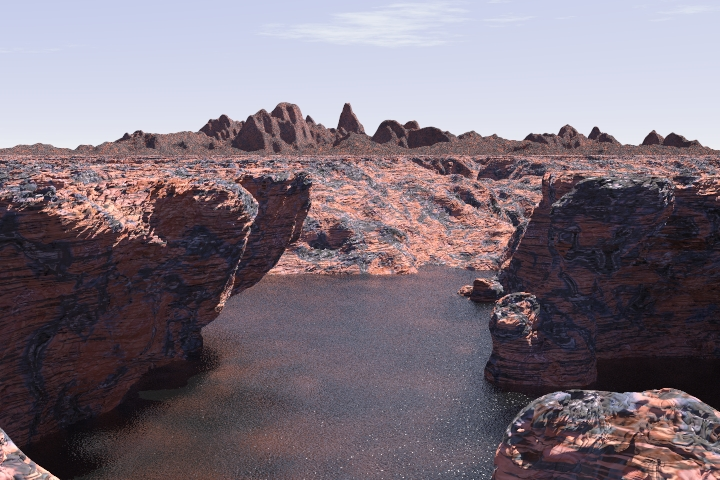
\includegraphics[width=0.7\textwidth]{img/mountain.jpg}
\caption{Detected corners with the Harris corner detector}
\label{fig:mountain}
\end{figure}

\begin{figure}[ht]
\centering
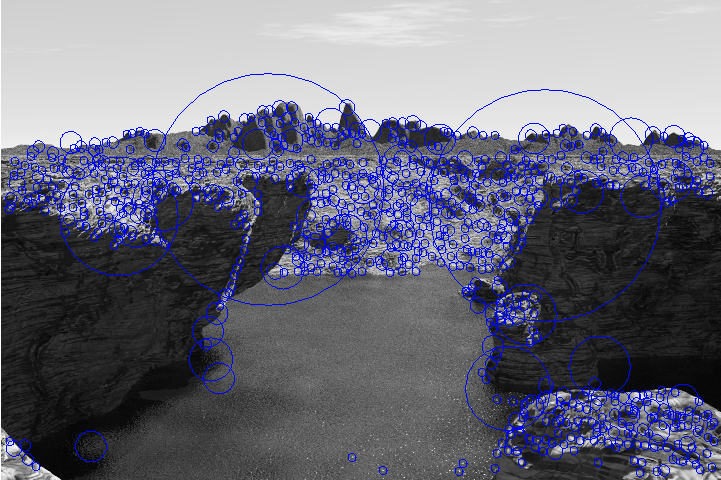
\includegraphics[width=0.7\textwidth]{img/Harris.png}
\caption{Detected corners with the Harris corner detector}
\label{fig:Harris}
\end{figure}

\section{Harris Laplace Corner Detector}

We also implemented the simplified Harris-Laplace detector as discussed by Mikolajczyk \cite{Miko}. This method follows the same approach as the Harris corner detector but for every points tests a finer range of sigmas thereby finding the local profile of the Laplacian. The extremum of the Laplacian can now be more accurately found. If the extremum is at the edge then the point is discarded as the extremum of the Laplacian lies on a different level. The same post processing step as applied in the Harris corner detector is used here. This method found 578 features. Results are shown in figure \ref{fig:HL}.


\begin{figure}[ht]
\centering
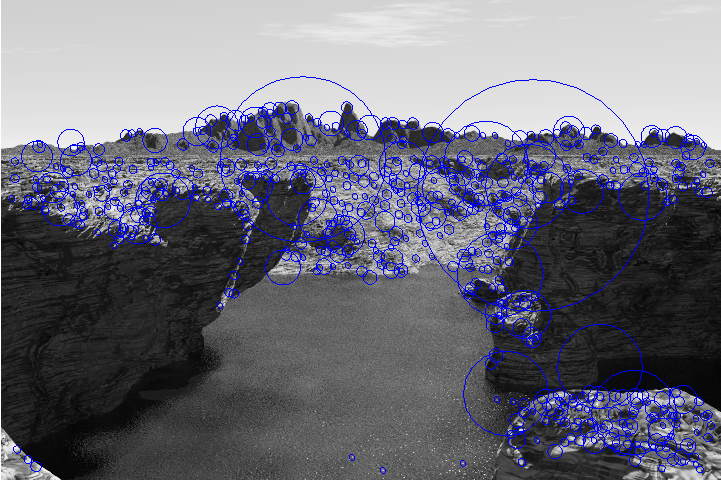
\includegraphics[width=0.7\textwidth]{img/HarrisLaplace.png}
\caption{Detected corners with the Harris-Laplace corner detector}
\label{fig:HL}
\end{figure}

\section{Difference of Gaussians Corner Detector}

A much faster implementation for corner detection is by estimating the Laplacian using difference of gaussians. The implementation was followed from David Lowes paper \cite{Lowe}. The Difference of gaussians is calculated in a scale space with the difference of gaussians defined as
\begin{equation}
D(x,y,\sigma) = (G(x,y,k\sigma) - G(x,y,\sigma)) * I(x,y)
\end{equation}
This approximates the Laplacian.\\
Next local extrema are detected by finding the local maxima in the 26 connected component neighbourhood of the scale space. If these local extrema have a respons bigger then a threshold ($D(x,y,\sigma) > 0.01$) then the detected point is not flat. But this filter is still very responsive to edges and so for every point the local variance components are checked by constructing the Hessian and checking the ratios of the eigen values (as described by Lowe \cite{Lowe}).\\
The total number of features detected by this method was 460. The result is shown in figure \ref{fig:DoG}

\begin{figure}[ht]
\centering
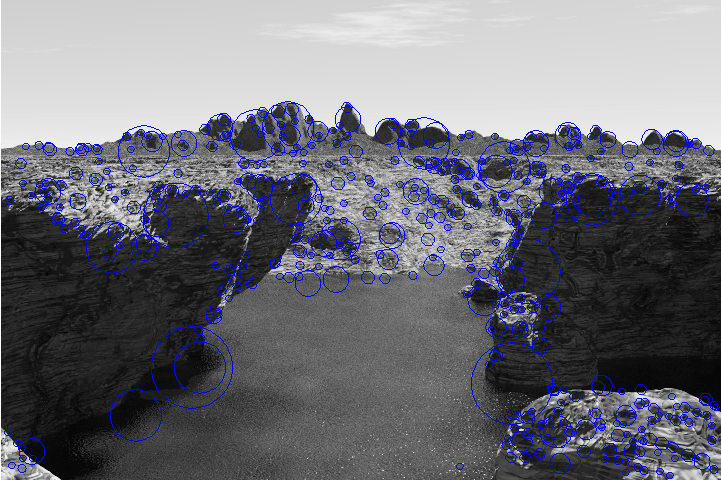
\includegraphics[width=0.7\textwidth]{img/DoG.png}
\caption{Detected corners using the DoG method}
\label{fig:DoG}
\end{figure}

\section{SIFT}
To match keypoints detected with the corner detection a descriptor is needed. David Lowes SIFT was used to create the SIFT descriptors for these keypoints. The VLFeat\footnote{http://www.vlfeat.org/} open source library was used. \\
For two images that show the same scene from different viewpoints, we find the corner points in both images and calculated the descriptor for them. Then the points are matched between the two images. The result can be seen in figure \ref{fig:matching} for the Harris Corner Points and in figure \ref{fig:matDoG} for the Difference of Gaussians.

\begin{figure}[ht]
\centering
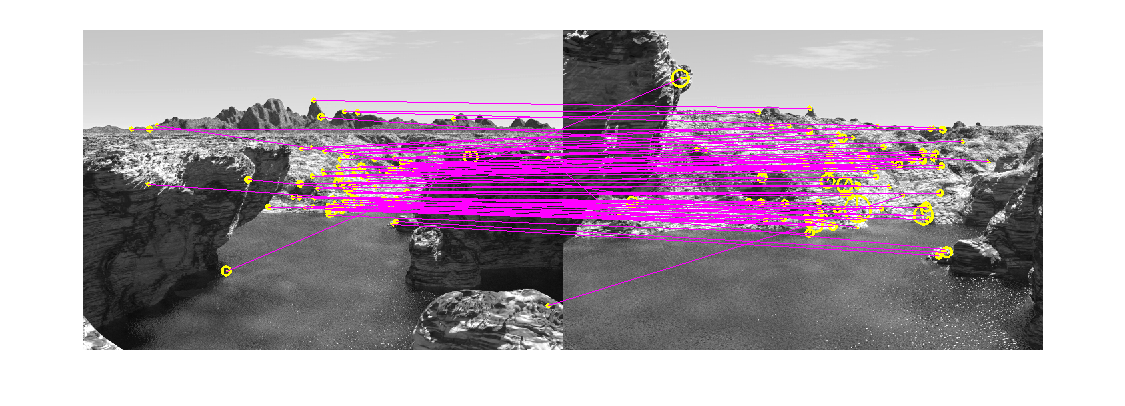
\includegraphics[width=\textwidth]{img/matchesLaplace.png}
\caption{Detected corners using the DoG method}
\label{fig:matching}
\end{figure}

\begin{figure}[ht]
\centering
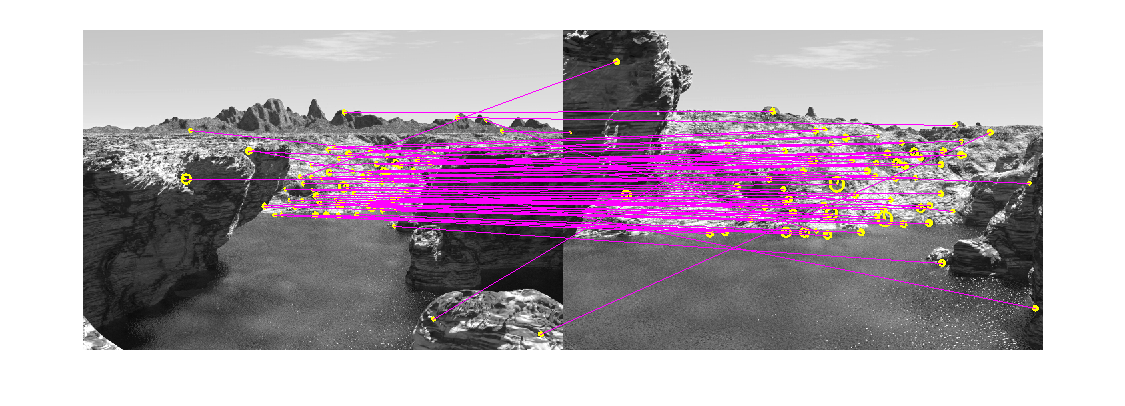
\includegraphics[width=\textwidth]{img/matchesDoG.png}
\caption{Detected corners using the DoG method}
\label{fig:matDoG}
\end{figure}

\bibliography{mybib}{}
\bibliographystyle{plain}

\end{document}

